\documentclass[a4paper,12pt]{article}

\author{Sofia B. Lopez}
\title{}

\usepackage[margin=0.9in]{geometry}
\usepackage{graphicx}
\usepackage{float}
\usepackage[utf8]{inputenc}
\usepackage[T2A]{fontenc}
\usepackage{textcomp}
\usepackage{amsmath, amssymb}
\usepackage{siunitx}

\begin{document}
\textbf{Число молекул \(n=125\)}\\
Молекулярная плотность $\rho=0.1$.
\begin{center}
  \begin{figure}[htb]
    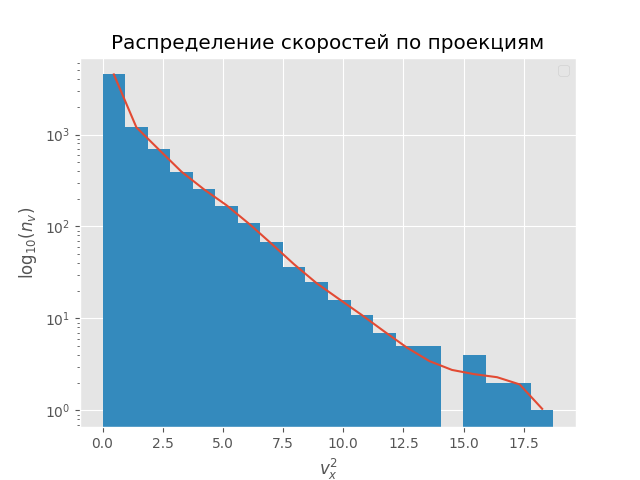
\includegraphics[width=0.6\textwidth]{hist1.png}
    \caption{Проверяем распределение скоростей по проециям для 20 испытаний (каждое испытание состоит из \(N=50000\) итераций с шагом \(dt=0.001\)).}
  \end{figure}
  \begin{figure}[htb]
    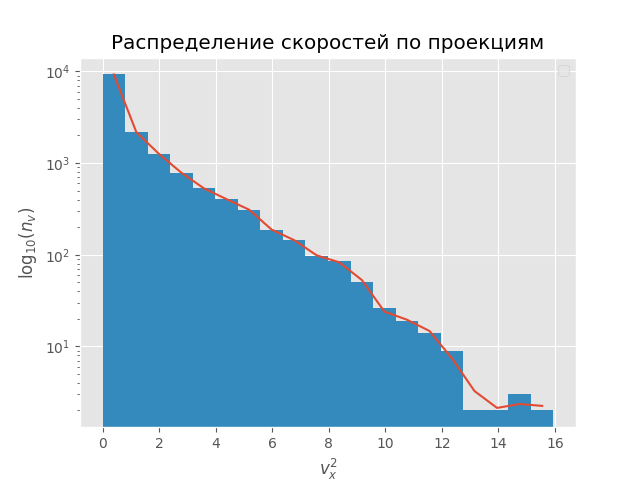
\includegraphics[width=0.6\textwidth]{hist2.png}
    \caption{Проверяем распределение скоростей по проециям для 41 испытаний (каждое испытание состоит из \(N=10000\) итераций с шагом \(dt=0.0001\)).}
  \end{figure}
\end{center}
\begin{center}
\end{center}
\begin{center}
  \begin{figure}[htb]
    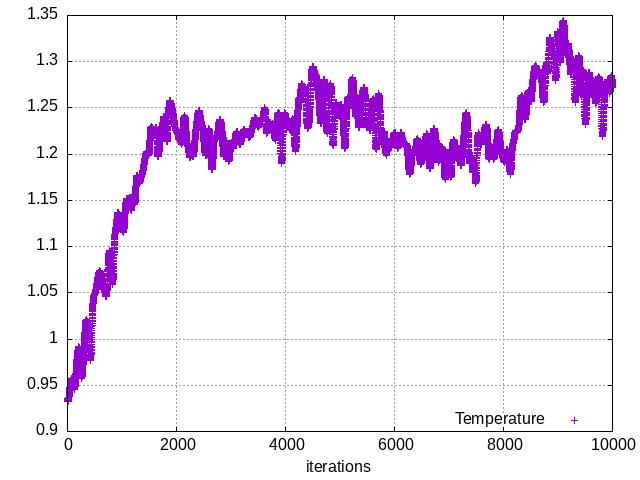
\includegraphics[width=0.7\textwidth]{g7_1.png}
    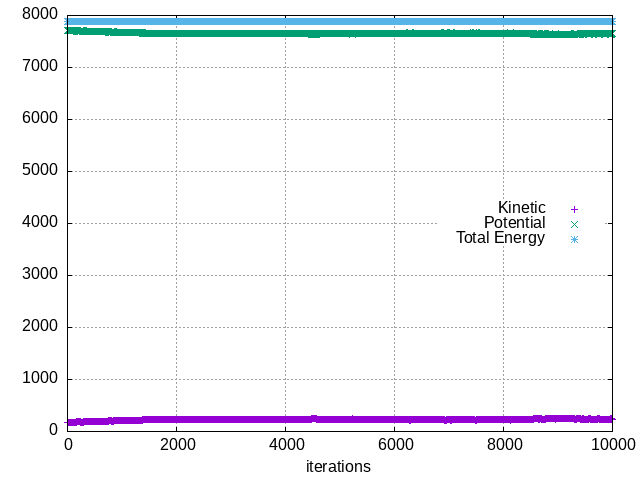
\includegraphics[width=0.7\textwidth]{g6_1.png}
  \end{figure}
\end{center}
\begin{center}
  \begin{figure}[htb]
    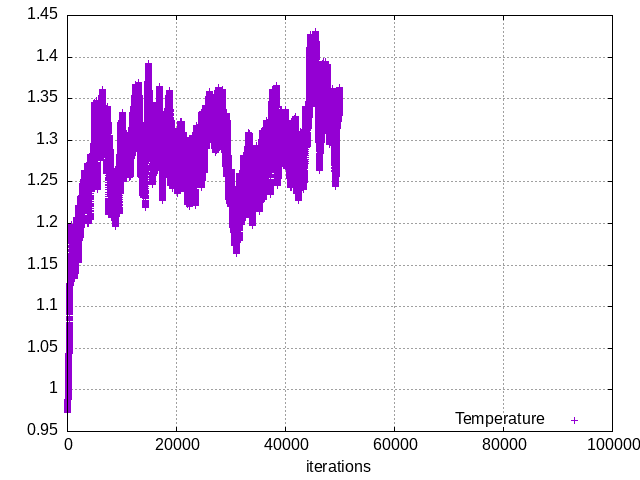
\includegraphics[width=0.7\textwidth]{g7.png}
    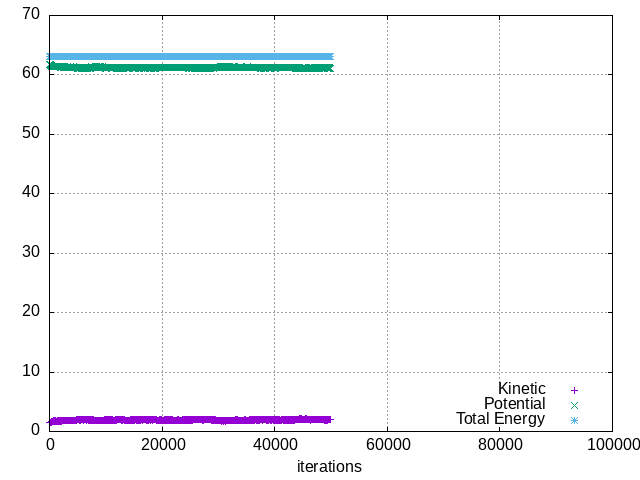
\includegraphics[width=0.7\textwidth]{g6.png}
  \end{figure}
\end{center}
\begin{center}
  \begin{figure}[htb]
    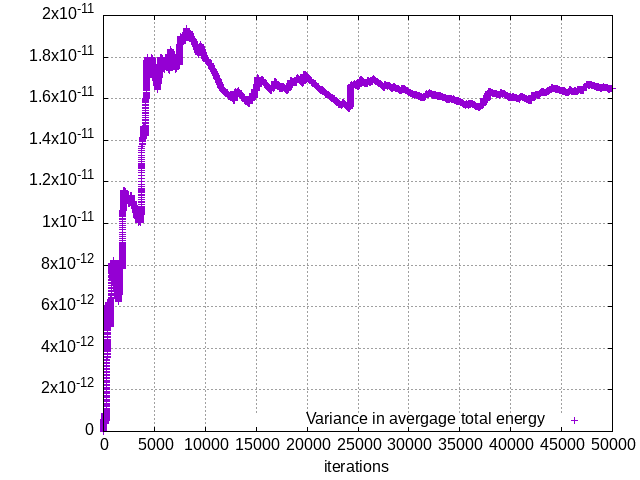
\includegraphics[width=0.7\textwidth]{g8.png}
    \caption{\(D=\frac{\sum(E_i-\overline{E})^2}{n-1}\)}
  \end{figure}
\end{center}
\end{document}
